\section{Global interval predicates and completion}\label{sec:descriptions}

We now describe each child as a global set without intersecting
with a recursively described parent. This is the step that converts
the construction into a polynomial family of subproblems.

\subsection{Global tests for local cutoffs}

The cutoff predicates in this section are used only in the final
interval and split formulas. The list construction and its entry-size
bound are now complete, so these formulas may retain the existing
bounded entries. The historical extension in \Cref{lem:old-low},
by contrast, had to flatten an earlier run before a new switch
entry could be constructed.

For every walk cutoff \(S\) in a parent \(W\), choose a global
predicate \(\widetilde S\) satisfying
\begin{equation}
 \widetilde S\cap W=S.
 \label{eq:cutoff-agreement}
\end{equation}
In the same case, let \(\K_{\mathrm{carry}}\) be the carry determined
by \(O\setminus S\), before the new injection. Use
\begin{equation}
 \widetilde S=P_b\setminus\Qual(\K_{\mathrm{carry}}).
 \label{eq:direct-same-cutoff}
\end{equation}
On \(W\), the carry selects precisely \(O\setminus S\), while
the low jobs are the initial \((W\setminus O)\cap P_b\) and the
promoted portion of \(O\). Thus \eqref{eq:cutoff-agreement} holds.
In the switch case use
\begin{equation}
 \widetilde S=(J\setminus D_a)\cap\{\rk\le r\},
 \label{eq:direct-switch-cutoff}
\end{equation}
where \(r\) is the rank of the last promoted member of \(X\),
or \(r=0\) before any promotion.
These formulas are available at every walk cutoff, whether or not
the associated open gap is nonempty.
They are not required to have any prescribed meaning outside \(W\).

\subsection{A child as a global set}

Figure~\ref{fig:gap} summarizes the localization steps in the following
formulas.

\begin{lemma}\label{lem:global-child}
In the valid construction of \Cref{prop:construction-valid}, let
\(W'=(a',b')\) be a child of \(W=(a,b)\), with parent center \(v\),
edge cutoff \(S\), new pruned list \(\K'\), and cutoff predicate
\(\widetilde S\) satisfying \eqref{eq:cutoff-agreement}.
In the edge's working frame, its high and low parts are the
following global sets:
\begin{align}
 W'\setminus S
 &=\Qual(\K')\cap P_{b'}\cap(J\setminus\wP{a'}),
 \label{eq:global-high}\\
 W'\cap S
 &=D_{a'}\cap P_b\cap(J\setminus\wD{b'})
                  \cap(J\setminus\wD v)\cap\widetilde S .
 \label{eq:global-low}
\end{align}
\end{lemma}
\begin{proof}
Every high child job qualifies, precedes \(b'\), and, because
it is later than \(a'\), is outside \(\wP{a'}\).
Conversely, a job selected by the right side of
\eqref{eq:global-high} is strictly before \(b'\) by precedence.
If it were at or before \(a'\), the child's global
Invariant~\ref{inv:past} would put it in \(\wP{a'}\).
It is therefore strictly in \(W'\), and the child list selects
exactly its high jobs.

For \eqref{eq:global-low}, consider first a job selected by its
right side. The two positive tests \(D_{a'}\cap P_b\) locate
it strictly inside the parent \(W\): its time is after
\(a'\ge a\) and before \(b\). This remains true with sentinel
boundaries under our conventions.
We can consequently use \eqref{eq:cutoff-agreement} to infer
that the job is in \(S\).
This cutoff is contained in the center-low set \(S_*\).
A selected job at or after \(v\) would therefore lie in
\(\wD v\), by the center separator or by membership in \(v\)
itself. The corresponding exclusion places it in the open side
\(E=(a,v)\).
Within \(E\), a low job at or after \(b'\) is in
\(\wD{b'}\), using the local separator at \(b'\).
The remaining exclusion puts the selected job strictly between
\(a'\) and \(b'\).

Conversely, a low job of this gap lies in \(D_{a'}\cap P_b\)
by \Cref{lem:edge-labels}, and it satisfies
\(\widetilde S\) by \eqref{eq:cutoff-agreement}.
Its time is strictly before both \(b'\) and \(v\), so it is
in neither of their weak successor cones. It passes every test
in \eqref{eq:global-low}.
\end{proof}

\begin{figure}[t]
\centering
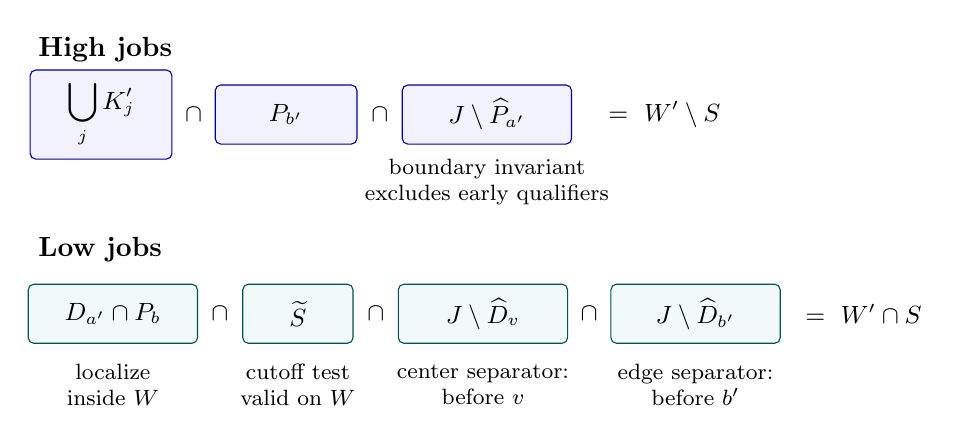
\begin{tikzpicture}[x=1cm,y=1cm,font=\small,
  filter/.style={draw,rounded corners=2pt,minimum height=.75cm,
                 minimum width=1.8cm,inner sep=4pt,align=center}]
  \node[anchor=west,font=\bfseries] at (-.92,2.18) {High jobs};
  \node[filter,draw=blue!60!black,fill=blue!5] (h1) at (0,1.35)
    {$\displaystyle\bigcup_j K'_j$};
  \node[filter,draw=blue!60!black,fill=blue!5] (h2) at (2.35,1.35)
    {$P_{b'}$};
  \node[filter,draw=blue!60!black,fill=blue!5,minimum width=2.15cm] (h3) at (4.9,1.35)
    {$J\setminus\widehat P_{a'}$};
  \node at (1.175,1.35) {$\cap$};
  \node at (3.54,1.35) {$\cap$};
  \node[anchor=west] at (6.32,1.35) {$=\ W'\setminus S$};
  \node[font=\footnotesize,align=center] at (4.9,.49)
    {boundary invariant\\excludes early qualifiers};

  \node[anchor=west,font=\bfseries] at (-.92,-.36) {Low jobs};
  \node[filter,draw=teal!65!black,fill=teal!5,minimum width=2.15cm] (l1) at (.15,-1.18)
    {$D_{a'}\cap P_b$};
  \node[filter,draw=teal!65!black,fill=teal!5,minimum width=1.4cm] (l2) at (2.5,-1.18)
    {$\widetilde S$};
  \node[filter,draw=teal!65!black,fill=teal!5,minimum width=2.15cm] (l3) at (4.85,-1.18)
    {$J\setminus\widehat D_v$};
  \node[filter,draw=teal!65!black,fill=teal!5,minimum width=2.15cm] (l4) at (7.55,-1.18)
    {$J\setminus\widehat D_{b'}$};
  \node at (1.51,-1.18) {$\cap$};
  \node at (3.49,-1.18) {$\cap$};
  \node at (6.20,-1.18) {$\cap$};
  \node[anchor=west] at (8.82,-1.18) {$=\ W'\cap S$};
  \node[font=\footnotesize,align=center] at (.15,-2.08)
    {localize\\inside $W$};
  \node[font=\footnotesize,align=center] at (2.5,-2.08)
    {cutoff test\\valid on $W$};
  \node[font=\footnotesize,align=center] at (4.85,-2.08)
    {center separator:\\before $v$};
  \node[font=\footnotesize,align=center] at (7.55,-2.08)
    {edge separator:\\before $b'$};
\end{tikzpicture}

\caption{The two global tests for a child.
For the low part, positive cones locate a candidate inside the parent
before its cutoff predicate is used; the two weak successor exclusions
then restrict that candidate to the gap.
For the high part, the global past-boundary invariant excludes
qualifiers at or before \(a'\).
The intersection factors are arranged in the order used by the proof.}
\label{fig:gap}
\end{figure}

The localization order matters. Neither the cutoff extension
\(\widetilde S\) nor the flattened historical extension needs to
agree with its intended local set everywhere in \(J\).
Positive cone tests first place the candidate in the domain where
agreement is known. The construction never appends a membership
predicate for all ancestor intervals.

\subsection{Relative predicates for the marked splits}

\begin{lemma}\label{lem:relative-splits}
Every marked slot \(z\) in a node \(W\) has a bounded relative
description of its earlier jobs in either the working direction
that produced it or the original direction. The formulas use the stated
atomic language and have fewer than \(500\) leaves, as counted in
\Cref{lem:final-count}.
\end{lemma}
\begin{proof}
Use the working frame for a side, and put
\[
 H_*=
 \begin{cases}
 P_b,&\same,\\
 J\setminus D_a,&\switch.
 \end{cases}
\]
For the center \(v\), the predicate \(B_v(H_*)\), restricted to
\(W\), is its earlier set, by
\Cref{lem:separator-description} and \eqref{eq:center-cutoff}.

For an internal mark \(z\) in the open side \(E\), choose a walk
cutoff \(S\) for which it is a local separator.
The predicate
\begin{equation}
 F_z=B_v(H_*)\cap B_z(\widetilde S)
 \label{eq:relative-split}
\end{equation}
gives its earlier set upon restriction to \(W\).
The first factor selects \(E\) on \(W\); on that domain the
second is the separator description from
\Cref{lem:separator-description}.

If the working frame is opposite to original time, \(F_z\cap W\)
describes the original \emph{later} jobs. Replace \(F_z\) by
\begin{equation}
 (J\setminus F_z)\setminus z
 \label{eq:reverse-split}
\end{equation}
to obtain the original earlier jobs after restriction to \(W\).
The exclusion of the marked triple is necessary: complementation
alone includes it. Apply the same conversion to the center
predicate when appropriate.
\end{proof}

\begin{lemma}\label{lem:final-count}
The predicates in \Cref{lem:global-child,lem:relative-splits}
have fewer than \(500\) leaves.
\end{lemma}
\begin{proof}
A pruned list or a carry contains at most five entries with fewer
than \(40\) leaves each, so its union has at most \(195\) leaves.
An empty union uses the false constant.
The same-direction cutoff \eqref{eq:direct-same-cutoff} therefore
needs at most \(196\) leaves; the switched one needs two.
Use \(205\) as a common loose allowance.

The high predicate \eqref{eq:global-high} uses at most
\(195+2=197\) leaves. The low predicate
\eqref{eq:global-low} uses at most \(205+4=209\).
Their union is a global description of \(W'\) with at most
\(406\) leaves.

The center predicate has three leaves. The internal split
\eqref{eq:relative-split} has at most \(3+(205+2)=210\),
and conversion \eqref{eq:reverse-split} adds one.
Complementation does not increase leaf counts.
Every cone uses an actual triple or a sentinel constant; all ranks
and thresholds are from the two allowed frames. Thus these are
formulas in the stated atomic language.
\end{proof}

\begin{proof}[Proof of \Cref{thm:structure}]
Use \Cref{prop:construction-valid} to construct marks and lists
from a feasible full schedule.
The root set \(J\) is represented by true.
Every nonempty child has the global description supplied by
\Cref{lem:global-child}. Every mark has the relative split
description supplied by \Cref{lem:relative-splits}.
\Cref{lem:final-count} places both kinds of description in
\(\F\), independently of their depth.
All branches terminate because the node sizes decrease strictly.
These are exactly the conditions of \Cref{def:hierarchy}.
\end{proof}
